\documentclass[12pt,oneside,justify]{book}

\usepackage[utf8]{inputenc}
\usepackage{mathptmx}
\usepackage{geometry}
\usepackage{fancyhdr}
\usepackage{tocloft}
\usepackage{titlesec}
\usepackage{textcomp}
\usepackage{pdfpages} 
\usepackage{graphicx}
\graphicspath{ {images/} }
\usepackage[
backend=biber,
]{biblatex}  % irodalomjegyzék

\titleformat{\chapter}{\normalfont\huge}{\thechapter.}{20pt}{\huge} % egyedi chapter szöveg

\geometry{
	a4paper,
	lmargin=3cm,
	tmargin=3cm,
	bmargin=3cm,
	rmargin=2cm
}

\fancyhead
\fancyfoot
\pagestyle{plain} % oldalstílus
\pagenumbering{arabic} % oldalszámozás 

\renewcommand{\headrulewidth}{0pt}
\renewcommand{\contentsname}{Tartalomjegyzék} % tartalomjegyzék átnevezés
\renewcommand{\listfigurename}{Ábrajegyzék} % ábrajegyzék átnevezés
\renewcommand\cftchapaftersnum{.} % chapter szám utáni pont
\renewcommand\cftchapdotsep{\cftdotsep} % chapter, és irodalomjegyzék szöveg utáni pontok

\addbibresource{bibliography.bib}

% help section - to be deleted

% \chapter{Második bekezdés}
% \section{másik bekezdés 2 szintű}
% \subsection{First Subsection}
% \paragraph{az}

% Ezt idéztem \cite{AzureFundamentals}

% \noindent // bekezdés első sorának indentálása

% end help section

\begin{document} 

\includepdf{outer_cover.pdf}
\includepdf{inner_cover.pdf}

\tableofcontents

\chapter{Virtualizáció}
\noindent Miért jó a virtualizáció. A virtualizált rendszerek előnyei. Modern virtualizációs megoldások
% \\TODO

\section{On-Premises rendszerek}

\subsection{Microsoft Hyper-V\texttrademark}

\subsubsection{Deduplikáció}

\noindent A Microsoft a Windows Server 2012 szerver verzióban jelentette be a Deduplikációt. A deduplikáció egy olyan folyamat amely feldolgozza az engedélyezett lemezek tartalmát és egyező adatblokkokat csak egyszer tárol le. Az ismétlődő blokkok esetén már csak referenciákat hagy. Ezzel a megoldással nagyon jó hatásfokkal lehet tárolóhelyet megtakarítani. A legjobban deduplikálható adatok a Virtualised Desktop Infrastructure - későbbiekben VDI rendszerek - amelyek esetén az operációs rendszer a hozzátartoztó frissítési csomagok, a feltelepített alkalmazások alapfileai többnyire minden rendszeren megegyeznek. Amennyiben a virtuális gépeken nagyon kevés egyedi file és telepített alkalmazás található úgy a deduplikációs ráta elérheti akár a 90\%-ot is.

%\\TODO kifejteni képekkel

\subsubsection{Virtual Network}

%\\TODO

\subsection{VMWare ESX \textsuperscript{\textregistered}}
\noindent

\subsection{Oracle\textsuperscript{\textregistered} VM}
\noindent

\section{Cloud megoldások}
\subsection{Microsoft Azure}
\noindent

\subsection{VMWare Cloud}
\noindent

\subsection{Oracle Cloud}
\noindent

\section{Platformok összehasonlítása}
\noindent

\chapter{Esettanulmány}
\section{Igényfelmérés}
\noindent

\section{Ajánlat}
\noindent

\section{Migráció cloudba}
\noindent

\chapter{Esettanulmány háttércég}

\section{Rendszer architektúra ismertetése}

\noindent Architektúrális szempontból Intel alapú szervereket használtam. A fejlesztői környezet alapját 2 db Dell PowerEdge R710-es szerver adta. A szerverek 
a munka ideje alatt egyenként 2 db Intel{\textsuperscript{\textregistered}} Xeon{\textsuperscript{\textregistered}} E6545 processzorral (6 mag 12 HT szál), 96 GB DDR3 ECC RAM-al, 2x64 GB Rendszer lemezekkel illetve 2x136 GB adatlemezzel volt ellátva. A kettő szerver egy failover clusterben üzemelt. A rendszer és az adat lemezek RAID1-ben üzemeltek az adatvesztés megelőzése és a magas rendelkezésre állás biztosítása érdekében. Az adatlemezek mérete sosem volt gond a Windows Deduplikációs megoldása miatt.

\subsubsection{A mester image használata}

\noindent A rendszereinket központilag nem menedzselt, de egységes alapkonfigurációval látjuk el annak érdekében, ha az ügyfélnek segítségre lenne szüksége. A mester image előállítása nagyban meggyorsítja a megrendelt rendszerek elkészítését. Alapvetően két nagy irányzatot lehet felismerni ezen megoldások terén. 

Az első megoldás amikor már egy telljesen kész rendszert tartalmazó de syspreppelt virtuális merevlemezt másolunk át a konténer mappájába. Majd azt a virtuális gép konfigurációjakor becsatoljuk és már indítható is rendszer. Ezek után összesen a végfelhasználó szerződést kell elfogadnunk és már használatba is vehetjük a gépünket. Amelyet át kell nevezni, be kell állítani számára a megfelelő IP konfigurációt és már át is adható a felhasználónak. 

A másik irányzat amikor a Microsoft Deployment Toolkitet használjuk. 
% \\TODO  A két irányzat alapvető lépéseit illetve a továbbiakban szükséges folyamatokat bemutatni
\begin{figure}[h]
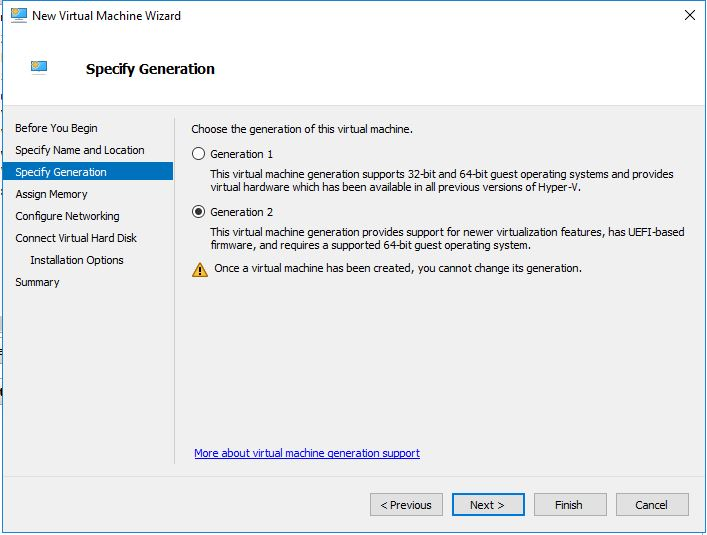
\includegraphics[width=\textwidth]{generation_selection}
\caption{Generáció választás Hyper-V managerből készített virtuális gép esetén}
\label{fig:gen_selection}
\end{figure}


\section{Automatizált megoldások}
\noindent

\subsection{On-prem}
\noindent
\subsubsection{Provision-ObjectsForCompany.ps1}
% \\TODO

\subsubsection{Create-VM.ps1}
% \\TODO

\subsubsection{Create-NewVirtualSwitch.ps1}
% \\TODO

\subsubsection{Post-Configuration.ps1}
% \\TODO

\subsection{Cloud}
\noindent

\chapter{PowerShell}
\section{Történelme}
% \\TODO
\section{Programozási paradigmák}
% \\TODO

\addcontentsline{toc}{chapter}{\listfigurename}
\listoffigures
\printbibliography[heading=bibintoc,title={Irodalomjegyzék}]
\end{document}
